\documentclass[article, a4paper, oneside, 12pt]{memoir}

\usepackage{listings}
\usepackage{xcolor-solarized}
\usepackage{inconsolata}
\usepackage{graphicx}
\lstset{
    language=Python,
    showstringspaces=false,
    backgroundcolor=\color{solarized-base3},
    commentstyle=\color{solarized-base1},
    stringstyle=\color{solarized-blue},
    keywordstyle=\color{solarized-cyan},
    basicstyle=\color{solarized-base00}\ttfamily,
    numberstyle=\color{solarized-violet},
    frame=lines,
    identifierstyle=\color{solarized-base00},
    sensitive=true,
    escapechar=\%
}

\usepackage{amsmath}
\usepackage{amsthm}
\usepackage{amssymb}
\usepackage{bm}
\usepackage{physics}
\usepackage{mathtools}
\usepackage{microtype}
\usepackage{geometry}
\linespread{1.25}

\usepackage{hyperref}
\usepackage{cleveref}

\DeclareMathOperator{\dist}{dist}
\DeclareMathOperator{\proj}{proj}
\DeclareMathOperator{\vect}{Vec}
\DeclareMathOperator{\Span}{Span}

\newcommand{\mat}[1]{\bm{#1}}
\newcommand{\frob}[1]{\norm{#1}_{\mathrm{F}}}

\title{\textsc{Mandatory Assignment 3 \\ 
MAT-INF4130}} 
\author{Ivar Stangeby}
\begin{document}
\maketitle 

\chapter{Introduction}        

Given a set of points \( \left\{\mat{x}_1, \ldots, \mat{x}_n\right\} \subseteq
\mathbb{R}^m \) and an integer \( k \leq m \), we are interested in finding the
\( k \)-dimensional subspace \( W \) that \emph{minimizes} the squared
distance:
\begin{equation}
    \sum_{i = 1}^m \dist(\mat{x}_i - W)^2.
\end{equation}

To this end we first establish some notation. Let \( \mat{X} \coloneqq
[\mat{x}_1, \ldots, \mat{x}_n]\) be the matrix with \(ij\)th element denoted
\(x_{ij} \).  If \( W \) is any \(k\)-dimensional subspace of \( \mathbb{R}^m
\) and \( \left\{ \mat{w}_j \right\}_{j=1}^k\) is an orthonormal basis for \( W
\), we may extend this basis to an orthonormal basis \( \left\{ \mat{w}_j
\right\}_{j=1}^m \) for \( \mathbb{R}^m \) by the Grahm-Schmidt algorithm. We
can therefore decompose the space \( \mathbb{R}^m \) into \( W \) and its
orthogonal complement \( W^\perp \):
\begin{equation}
    \mathbb{R}^m = W \oplus W^\perp.
\end{equation}
For a vector \( \mat{x} \in \mathbb{R}^m\), denote by \(
\proj_{W^\perp}(\mat{x}) \), its orthogonal projection onto \( W^\perp \).
Furthermore, recall that the Frobenius norm of a matrix \( \mat{A} \in
\mathbb{C}^{m\times n}\) is defined as:
\begin{equation}
    \frob{\mat{A}} \coloneqq \left( \sum_{i=1}^m \sum_{j=1}^n |a_{ij}|^2 \right)^{1/2}
\end{equation}
and that this is equivalent to the 2-norm of the vector \( \vect(\mat{A}) \)
formed by stacking the columns of \( \mat{A} \) on top of each other.  We
denote by \( \langle \cdot, \cdot \rangle \) the standard inner product on
\( \mathbb{R}^m \) defined by
\( \langle \mat{x}, \mat{y} \rangle \coloneqq \mat{y}^T \mat{x} \).

\chapter*{Exercise 1}

We start by showing that 
\begin{equation}
    \label{eq:proj_goal}
    \sum_{i=1}^n \norm{\proj_{W^\perp} (\mat{x}_i)}^2_2 = \frob{\mat{X}^T\mat{W}}^2.
\end{equation}
where \( \mat{W} \) is the \( m \times (m - k) \) matrix defined as \( \mat{W}
\coloneqq [\mat{w}_{k+1}, \ldots, \mat{w}_{m}] \).
Since \( \left\{ \mat{w}_{k+1}, \ldots, \mat{w}_{m} \right\} \) is a basis for
\( W^\perp \), we can write \( \proj_{W^\perp} (\mat{x}_i) = \sum_{j = k + 1}^m
c_i \mat{w}_i \) where \( c_j = \langle \mat{x}_i, \mat{w}_j \rangle \).
Expanding the left hand side of \cref{eq:proj_goal} yields:
\begin{align}
    \begin{split}
        \sum_{i=1}^n \norm{\proj_{W^\perp} (\mat{x}_i)}^2_2 &= \sum_{i = 1}^n \langle
        \proj_{W^\perp}(\mat{x}_i), \proj_{W^\perp}(\mat{x}_i) \rangle \\ 
        &= \sum_{i = 1}^n \sum_{j = k+1}^m \sum_{\ell = k+1}^m \langle \mat{x}_i, \mat{w}_j \rangle \langle \mat{x}_i, \mat{w}_{\ell} \rangle \delta_{j, \ell} \\
        &= \sum_{i = 1}^n \sum_{j=k+1}^m |\langle \mat{x}_i, \mat{w}_j \rangle|^2.
    \end{split}
\end{align}
Since we are working over the reals, we may write \( \langle \mat{x}_i,
\mat{w}_j  \rangle = \langle \mat{w}_j, \mat{x}_i \rangle \), hence the
equality follows in \cref{eq:proj_goal}.

\chapter*{Exercise 2}

Let \( \mat{X} = \mat{U}\mat{\Sigma}\mat{V}^T \) be a singular value
decomposition of \( \mat{X} \). 
\begin{enumerate}[a)]
    \item We wish to show that
\begin{equation}
    \frob{\mat{X}^T \mat{W}}^2 = \frob{\mat{\Sigma}^T\mat{U^T}\mat{W}}^2.
\end{equation}
This can easily be shown by noting that for arbitrary unitary matrix \( \mat{B}
\) and matrix \( \mat{A} \) we  have
\begin{equation}
    \label{eq:frob_unitary}
    \frob{\mat{BA}} = \frob{\mat{A}}.
\end{equation}
This follows from the fact that the Frobenius norm on \( \mathbb{C}^{m\times n}
\) is the same as the 2-norm on the vector space \( \mathbb{C}^{mn} \) and that
\( \norm{\mat{Bx} }_2 = \norm{ \mat{x} }_2 \) for all \( \mat{x} \).  Indeed, we
have
\begin{align}
    \frob{\mat{BA}} = \sum_{j = 1}^n \norm{ \mat{Ba}_{:j}}_2 = \sum_{j = 1}^n \norm {
    \mat{a}_{:j} }_2 = \frob{\mat{A}}.
\end{align}
Setting \( \mat{B} \coloneqq \mat{V} \) and \( \mat{A} \coloneqq \mat{\Sigma^T
U^T W}\) in \cref{eq:frob_unitary} and squaring proves the result.  

\item We now wish
to show that
\begin{equation}
    \frob{\mat{X}^T\mat{W}} = \sum_{i=1}^m
    \sigma_i^2\|\proj_{W^\perp}(\mat{u}_i)\|_2^2
\end{equation}
Expanding the matrix \( \mat{U}^T\mat{W} \) tells us that the \(ij\)th entry is
given by
\begin{equation}
    (\mat{U}^T\mat{W})_{ij} = \langle \mat{u}_i, \mat{w}_{j + k}\rangle
\end{equation}
for \( i = 1, \ldots, m \) and \( j = 1, \ldots, m - k \). Pre-multiplying by
\( \mat{\Sigma}^T \) gives
\begin{equation}
    (\mat{\Sigma}^T\mat{U}^T\mat{W})_{ij} = \sigma_i \langle \mat{u}_i, \mat{w}_{j+k} \rangle
\end{equation}
We can therefore write the Frobenius norm of this matrix as
\begin{align*}
    \frob{\mat{\Sigma}^T\mat{U}^T\mat{W}}^2 = \sum_{i=1}^m \sigma_i^2
    \sum_{j=1}^{m-k} \langle \mat{u}_i, \mat{w}_{j+k}\rangle  = \sum_{i=1}^m
    \sigma_i^2 \norm{\proj_{W^\perp}(\mat{u}_i)}_2^2
\end{align*}
as we wanted to show. Note that the singular values are ordered by convention
\( \sigma_1 \geq \ldots \sigma_m \geq 0 \).


\item We also have the property that since the columns of \( \mat{W} \) are
    orthonormal, and since there are \( m - k \) such columns, that 
\begin{equation}
    \frob{\mat{W}}^2 = m - k.
\end{equation}
Since \( \mat{U}^T \) is unitary, we have that
\begin{align}
    \frob{\mat{W}}^2 = \frob{\mat{U}^T\mat{W}}^2 = \sum_{i=1}^m \sum_{j=k+1}^m \langle \mat{u}_i, \mat{w}_j \rangle^2 = \sum_{i=1}^m \norm{\proj_{W^\perp}(\mat{u}_i)}^2_2.
\end{align}
\end{enumerate}
\chapter*{Exercise 3}
\begin{enumerate}[a)]
    \item We can now find the ``distance to the best subspace'' \(
        \frob{\mat{X}^T\mat{W}}^2 \) by solving the minimization problem
        \begin{equation}
            \min \sum_{i=1}^m \sigma_i^2 \kappa_i
        \end{equation}
        where \( 0 \leq \kappa_i \leq 1 \) and \( \sum_{i=1}^m \kappa_i = m - k \).
        Indeed, we have
        \begin{equation}
            \frob{\mat{X}^T\mat{W}}^2 = \sum_{i = 1}^m \sigma_i^2 \norm{\proj_{W^\perp}(\mat{u}_i)}^2_2
        \end{equation}
        where setting \( \kappa_i \coloneqq \norm{\proj_{W^\perp}(\mat{u}_i)}_2^2 \)
        yields the above sum. Furthermore, we have that \( 0 \leq \kappa_i \leq 1 \)
        since the \( \mat{u}_i\)'s are orthonormal, and we showed above that \(
        \sum_{i=1}^m \kappa_i = m - k \).

\item The solution to this problem is obtained by setting \( \kappa_1 = \ldots
    = \kappa_k = 0 \) and \( \kappa_{k+1} = \ldots = \kappa_{m} = 1 \), since
    the \( \sigma_i\)'s are ordered by magnitude. Indeed, the sum is minimized
    if we chose the vectors such that the columns of \( \mat{W} \) are
    perpendicular to \( \Span({\mat{u_1}, \ldots, \mat{u}_k}) \). Since \( 0
    \leq \kappa_i \leq 1 \), this means in order for \( \sum_{i = 1}^m = m - k
    \), we must have \( \kappa_{k+1} = \ldots = \kappa_{m} = 1\).

\item We can therefore choose the matrix \( \mat{W} \) to consist of the last
    \( m - k \) vectors \( \mat{u}_{k+1}, \ldots, \mat{u}_{m} \) and let \(
    W^\perp = \Span(\mat{u}_{k+1}, \ldots, \mat{u}_m) \). This set of vectors
    satisfies the minimization problem discussed above.  
    
\item We implement a routine for solving this minimization problem in
    \textsc{Python}. 

\begin{lstlisting}{language=Python}
def bestfit(X, k):
    U = np.linalg.svd(X)[0]
    B = U[:, :k]
    W = U[:, k:]
    dist = np.linalg.norm(X.T.dot(W))
    return B, dist
\end{lstlisting}
\end{enumerate}
\chapter*{Exercise 4}

We can alternatively choose to implement a ``vanilla'' least squares, where we
view the first \( k \) components of each column in \( \mat{X} \) as input data
and the last \( m - k \) components of each column as output data. By defining
\( \mat{Y} \coloneqq \mat{X}_{1:k, 1:n} \) and \( \mat{Z} \coloneqq
\mat{X}_{k+1:m, 1:n} \), we seek the matrix \( \mat{A} \) that minimizes
\begin{equation}
    \frob{\mat{AY}-\mat{Z}}.
\end{equation}
\begin{enumerate}[a)]
    \item It can be shown that if \( \mat{A} \) solves the least squares problem, then it
must satisfy the relation
\begin{equation}
    \mat{A}^T = (\mat{YY^T})^{-1} \mat{YZ}^T,
\end{equation}
however I was not successful in proving this.

\item 
We implement vanilla least squares in \textsc{Python}:
\begin{lstlisting}{language=python}
def vanleastsqr(X, k):
    Y = X[0:k, 0:]
    Z = X[k:, 0:]
    A = la.inv(Y.dot(Y.T)).dot(Y).dot(Z.T).T
    dist = la.norm(A.dot(Y) - Z)
    return A, dist
\end{lstlisting}
\end{enumerate}

\section*{Exercise 5}

The two algorithms previously discussed are tested on two test \( 2 \times 21
\) matrices \( \mat{X}_0 \) and \( \mat{X}_1 \). The first row of matrix \(
\mat{X}_1 \) contains 21 uniformly spaced values between -1 and 1, while the
second row contains uniformly random numbers between -1 and 1. All the elements
in \( \mat{X}_2 \) are random.

As we see from
\cref{fig:result}, the ``bestfit'' algorithm provides a better fit in both
cases. This might be due to numerical instability in the computation of the
inverse in the vanilla least squares.

\begin{figure}[htbp]
    \centering
    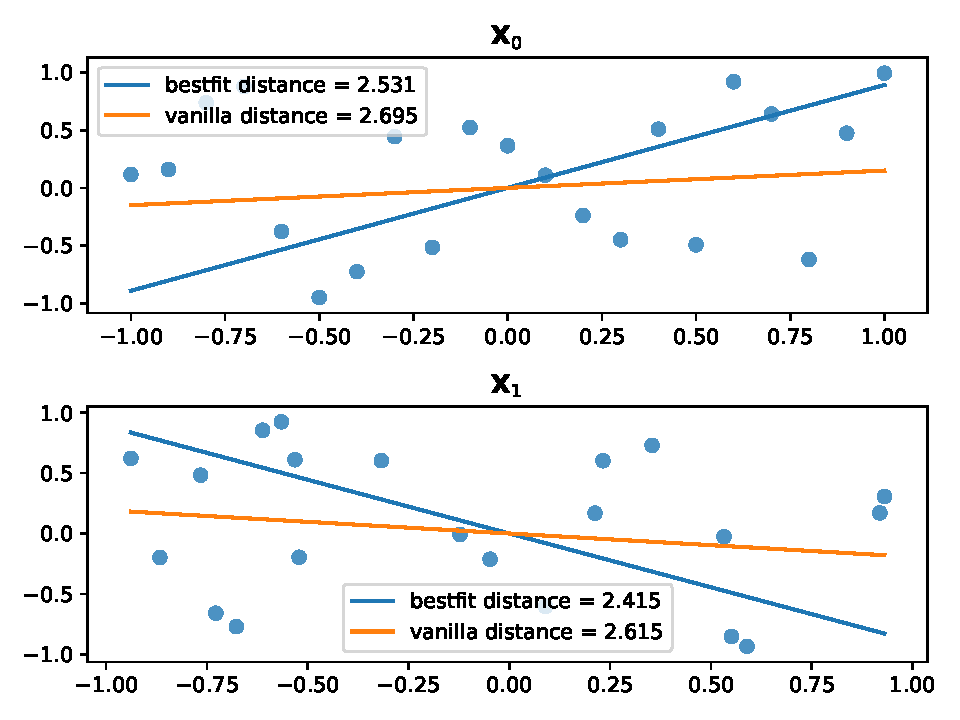
\includegraphics[width=0.8\linewidth]{pictures/best_subspace.pdf}
    \caption{Two approaches to the least squares problem of finding the best
    subspace. As we see, the fit is better for the ``bestfit'' algorithm, in
both cases.}
    \label{fig:result}
\end{figure}
\end{document}
